\subsection{Resumen de la din\'amica del aut\'omata celular}
\label{subsec-resumen}
En las secciones~\ref{subsec-celldiv}, \ref{subsec-migrant}, \ref{subsec-migration}, \ref{subsec-metastasis}, \ref{subsec-micrometastasis} y \ref{subsec-dormancy} se expuso el proceso gradual de concepci\'on de la din\'amica del aut\'omata celular, basada en dos componentes fundamentales: el conjunto de reglas y en el procedimiento de actualizaci\'on. Como el t\'itulo de esta secci\'on lo indica se presenta una recapitulaci\'on final de estos componentes fundamentales antes de pasar a las tareas de an\'alisis de resultados y validaci\'on del modelo. 

\subsubsection{Procedimiento de actualizaci\'on}
Dada la naturaleza de las distintas entidades biol\'ogicas que se recogen en el presente modelo de aut\'omatas celulares, presentadas en la secci\'on~\ref{subsec-states}, no es posible implementar el procedimiento cl\'asico de actualizaci\'on s\'incrona en el que se aplica la funci\'on de transici\'on local a todas las c\'elulas del aut\'omata de forma simult\'anea. Como se expuso a lo largo de la secci\'on~\ref{subsec-migration} se adopta un enfoque h\'ibrido en el que cada tipo de c\'elula es tratada seg\'un su propia naturaleza y las reglas del aut\'omata que rigen su comportamiento. En el cuadro~\ref{table-update-set} se muestran los conjuntos de actualizaci\'on definidos mostrando los tipos de c\'elulas contenidas en los mismos y el modo en que se llevan a cabo, es decir, de forma s\'incrona o as\'incrona. En adici\'on a estos conjuntos se definen un n\'umero de par\'ametros que cumplen un papel fundamental en el procedimiento de actualizaci\'on, como se muestra en el cuadro~\ref{table-update-params}. Finalmente el procedimiento de actualizaci\'on y cada uno de los m\'etodos que lo componen se muestran en los algoritmos~\ref{alg-update-r}, \ref{alg-update-r-1}, \ref{alg-update-r-2}, \ref{alg-update-r-3}, \ref{alg-update-r-4}, \ref{alg-update-r-5} y \ref{alg-update-r-6} respectivamente. Para m\'as informaci\'on verifique las reglas del aut\'omata celular presentadas posteriormente.

\begin{table}[h!]
\begin{center}
\scalebox{0.9}{\begin{tabular}{|p{2cm}|p{14.5cm}|} \hline
\emph{Par\'ametro} & \emph{Descripci\'on} \\\hline
\multicolumn{1}{|c|}{$C^S(G)$} & Conjunto de actualizci\'on s\'incrono. Contiene a las c\'elulas normales correspondientes con el lumen (estado $0$), el epitelio (estado $1$) y el estroma (estado $2$), as\'i como a las c\'elulas tumorales (estado $3$) que no poseen conexiones distantes y las c\'elulas de las micromet\'astasis (estado $5$). \\\hline
\multicolumn{1}{|c|}{$C_{mig}^A(G)$} & Conjunto de actualizaci\'on as\'incrono. Contiene a las c\'elulas migratorias del c\'ancer (estado $4$). \\\hline
\multicolumn{1}{|c|}{$C_{sc}^A(G)$} & Conjunto de actualizaci\'on as\'incrono. Contiene a las c\'elulas migratorias del c\'ancer que residen en el sistema circulatorio. \\\hline
\multicolumn{1}{|c|}{$C_{tum}^S(G)$} & Conjunto de actualizaci\'on s\'incrono. Contiene a las c\'elulas tumorales (estado $3$) que poseen conexiones distantes. \\\hline
\end{tabular}}\vspace*{-0.5cm}
\end{center}
\caption[Resumen de los conjuntos utilizados en el procedimiento de actualizaci\'on]{Resumen de los conjuntos utilizados en el procedimiento de actualizaci\'on.}
\label{table-update-set}
\end{table}

\begin{table}[h!]
\begin{center}
\scalebox{0.9}{\begin{tabular}{|p{2cm}|p{14.5cm}|} \hline
\emph{Par\'ametro} & \emph{Descripci\'on} \\\hline
\multicolumn{1}{|c|}{$\psi_{mig}$} & Probabilidad de la c\'elula migratoria de llevar a cabo un desplazamiento. \\\hline
\multicolumn{1}{|c|}{$\mu_{mig}$} & Cantidad de movimientos tentativos que la c\'elula migratoria puede llevar a cabo en un instante de tiempo.\\\hline
\multicolumn{1}{|c|}{$\xi_{sc}$} & Probabilidad de supervivencia de una c\'elula migratoria durante el transporte en el sistema circulatorio.\\\hline
\multicolumn{1}{|c|}{$\psi_{met0}$, $\psi_{met1}$} & Probabilidad de la c\'elula migratoria de arribar al \'organo destino correspondiente. \\\hline
\multicolumn{1}{|c|}{$\xi_{mic}$} & Probabilidad de supervivencia de una micromet\'astasis.\\\hline
\multicolumn{1}{|c|}{$\psi_{mic}$} & Probabilidad de colonizaci\'on de una micromet\'astasis.\\\hline
\end{tabular}}\vspace*{-0.5cm}
\end{center}
\caption[Resumen de los par\'ametros del procedimiento de actualizaci\'on]{Resumen de los par\'ametros del procedimiento de actualizaci\'on.}
\label{table-update-params}
\end{table}

\begin{algorithm}[h!]
\caption{Implementaci\'on del procedimiento de actualizaci\'on del aut\'omata celular.} \label{alg-update-r}
\KwData{$C_{mig}^A(G),\,C_{sc}^A(G),\,C_{tum}^S(G),\,C^S(G),\,S(n),\,\psi_{mig},\,\mu_{mig},\,\xi_{sc},\,\psi_{met0},\,\psi_{met1},\,\xi_{mic},\,$ $\psi_{mic},\,L_{mic}(n)$}
$update-migratory-cells-in-bloodstream(C_{sc}^A(G),\,\psi_{met0},\,\psi_{met1},\,\xi_{sc})$\;
$update-migratory-cells(G,\,C_{mig}^A(G),S(n),\,\psi_{mig},\,\mu_{mig})$\;
$update-tumor-migratory-cells(G,\,C_{tum}^S(G),\,C_{sc}^A(G),\,S(n))$\;
$check-micrometastasis-survival(L_{mic}(n),\,S(n),\,\xi_{mic})$\;
$update-synchronous-cells(G,\,C_{sc}^A(G),\,C^S(G),\,S(n))$\;
$check-micrometastasis-colonization(L_{mic}(n),\,S(n),\,\psi_{mic})$\;
\end{algorithm}

\begin{algorithm}[h!]
\caption{Implementaci\'on del m\'etodo $update-migratory-cells-in-bloodstream$ $(C_{sc}^A(G),\,\psi_{met0},\,\psi_{met1},\,\xi_{sc})$ encargado de la actualizaci\'on del conjunto as\'incrono que contiene a las c\'elulas migratorias contenidas en el torrente sangu\'ineo.} \label{alg-update-r-1}
\KwData{$C_{sc}^A(G),\,\xi_{sc},\,\psi_{met0},\,\psi_{met1}$}
\While{$|C_{sc}^A(G)|~\neq~0$}{
	$v=select-random-vertex(C_{sc}^A(G))$\;
	$w=get-target-vertex(v,\,C_{sc}^A(G))$\;
	$\psi=get-target-organ-probability(w,\,\psi_{met0},\,\psi_{met1})$\;
	\If{$random(0,1) \leq \xi_{sc} \wedge random(0,1) \leq \psi \wedge s(w,n) = 2$}{		
		$create-new-metastasis(w)$\;}
	$remove-cell-from-bloodstream(v,\,C_{sc}^A(G))$\;}
\end{algorithm}

\begin{algorithm}[p]
\caption{Implementaci\'on del m\'etodo $update-migratory-cells(G,\,C_{mig}^A(G),\,S(n),$ $\psi_{mig},\,\mu_{mig})$ encargado de la actualizaci\'on del conjunto as\'incrono que contiene a las c\'elulas migratorias.} \label{alg-update-r-2}
\KwData{$G,\,C_{mig}^A(G),\,S(n),\,\psi_{mig},\,\mu_{mig}$}
$updated=\lbrace \rbrace$\;
$i=0$\;
\While{$i < \mu_{mig}$}{
	\While{$|C_{mig}^A(G)|~\neq~|updated|$}{
		\Repeat{$v \notin updated$}{
			$v=select-random-vertex(C_{mig}^A(G))$\;}
		\If{$random(0,1) \leq \psi_{mig}$}{
			$apply-local-transition-function(v,\,S(n),\,G)$\;}
		$updated = updated \cup v$\;}
	$updated=\lbrace \rbrace$\;	
	$i++$\;}
\end{algorithm}

\begin{algorithm}[p]
\caption{Implementaci\'on del m\'etodo $update-tumor-migratory-cells(G,\,$ $C_{tum}^S(G),\,C_{sc}^A(G),\,S(n))$ encargado de la actualizaci\'on del conjunto as\'incrono que contiene a las c\'elulas tumorales que est\'an en presencia de una conexi\'on distante y cuya descendencia migratoria tiene la posibilidad de penetrar el sistema circulatorio.} \label{alg-update-r-3}
\KwData{$G,\,C_{tum}^S(G),\,C_{sc}^A(G),\,S(n)$}
\For{$v \in C_{tum}^S(G)$}{
	$p=get-probability(v)$\;
	\If{$random(0,1) \leq p$}{
		$d=select-destiny-vertex(v,\,S(n),\,G)$\;
		$add-cell-to-bloodstream(v,\,d,\,C_{sc}^A(G))$\;}}
\end{algorithm}

\begin{algorithm}[p]
\caption{Implementaci\'on del m\'etodo $check-micrometastasis-survival(L_{mic}(n),\,$ $S(n),\,\xi_{mic})$ encargado de verificar la supervivencia de las micromet\'astasis en el nuevo entorno a colonizar.} \label{alg-update-r-4}
\KwData{$L_{mic}(n),\,S(n),\,\xi_{mic}$}
\For{$l \in L_{mic}(n)$}{
	\If{$random(0,1) \leq 1 - \xi_{mic}$}{
		\For{$v \in l$}{
			$set-cell-status(S(n),\,v,\,2)$\;}}}
\end{algorithm}

\begin{algorithm}[h!]
\caption{Implementaci\'on del m\'etodo $update-synchronous-cells(G,\,C^S(G),\,S(n))$ encargado de la actualizaci\'on del conjunto s\'incrono que contiene a las c\'elulas normales, tumorales y las pertenecientes a las micromet\'astasis.} \label{alg-update-r-5}
\KwData{$G,\,C^S(G),\,S(n)$}
\For{$v \in C^S(G)$}{
	$apply-local-transition-function(v,\,S(n),\,G)$\;}
\end{algorithm}

\begin{algorithm}[h!]
\caption{Implementaci\'on del m\'etodo $check-micrometastasis-colonization$ $(L_{mic}(n),\,S(n),\,\psi_{mic})$ encargado de verificar la colonizaci\'on satisfactoria del entorno por parte de las micromet\'astasis.} \label{alg-update-r-6}
\KwData{$L_{mic}(n),\,S(n),\,\psi_{mic}$}
\For{$l \in L_{mic}(n)$}{
	\If{$random(0,1) \leq \psi_{mic}$}{
		\For{$v \in l$}{
			$set-cell-status(S(n),\,v,\,3)$\;}}}
\end{algorithm}

\subsubsection{Conjunto de reglas}
Como se expuso en la definici\'on~\ref{def-automata}, la funci\'on de transici\'on local se expresa mediante reglas que determinan el estado de una c\'elula en el siguiente instante de tiempo a partir del estado de las c\'elulas vecinas. En la secci\'on~\ref{subsec-function} se mostr\'o que en la funci\'on de transici\'on se destacan dos componentes fundamentales: el criterio de selecci\'on de la regla que se basa en el estado de la configuraci\'on local, y la probabilidad de transici\'on que tambi\'en depende de dicha configuraci\'on local en el sentido cl\'asico. Ante la necesidad de representar procesos complejos que dependen de un n\'umero mayor de factores, como el crecimiento tumoral o la migraci\'on de c\'elulas cancer\'igenas, en el presente modelo se adoptan una serie de extensiones en las que el criterio de selecci\'on de la regla permanece de acuerdo a la definici\'on cl\'asica de un aut\'omata celular pero la probabilidad de transici\'on se hace depender de nuevos factores y variables. En la secci\'on~\ref{subsec-celldiv} se indica que las reglas del aut\'omata encargadas de reproducir el crecimiento tumoral se infieren a partir de un modelo continuo, en este caso, la ley de crecimiento log\'istico de Verhulst, haciendo de la poblaci\'on tumoral una variable fundamental en el trabajo. Por tanto, las dem\'as reglas del aut\'omata encargadas de reproducir la aparici\'on de c\'elulas migratorias o el crecimiento de una micromet\'astasis tambi\'en la utilizan. Con el objetivo de dar una visi\'on completa de la concepci\'on del aut\'omata comenzamos recapitulando con las hip\'otesis en las que se basa el presente modelo:

\begin{enumerate}
\item [{I.}] \textbf{Progresi\'on idealizada del desarrollo tumoral}: \emph{Se asume que el desarrollo tumoral sigue una progresi\'on idealizada dividida en las etapas avascular y vascular, donde el comportamiento macrosc\'opico del tumor est\'a definido por las mutaciones que expresan las c\'elulas cancer\'igenas.} \label{hI}

\item [{II.}] \textbf{Mutaciones de las c\'elulas cancer\'igenas}: \emph{Se asume que la acumulaci\'on de mutaciones en la c\'elula cancer\'igena se define como un proceso secuencial y sigue un orden establecido, es decir, durante la etapa avascular se expresan las mutaciones relacionadas con el ciclo celular y la proliferaci\'on tumoral, y durante la etapa vascular se expresan las mutaciones relacionadas con la angiog\'enesis y met\'astasis, en adici\'on a las anteriores.} \label{hII}

\item [{III.}] \textbf{Entidades biol\'ogicas del modelo}: \emph{Las entidades biol\'ogicas presentes en el modelo se componen \'unicamente de los tipos de c\'elulas definidos en el conjunto de estados del aut\'omata celular.} \label{hIII}

\item [{IV.}] \textbf{Interacciones entre las entidades del modelo}: \emph{Las interacciones entre las distintas c\'elulas del modelo se compone solamente por las reglas definidas en la funci\'on de transici\'on del aut\'omata.} \label{hIV}

\item [{V.}] \textbf{Invarianza de las c\'elulas normales}: \emph{Se asume que la poblaci\'on de c\'elulas normales del organismo es est\'atica e invariante durante el transcurso del tiempo, es decir, no incurren en los procesos de divisi\'on ni muerte celular.} \label{hV}

\item [{VI.}] \textbf{Homogeneidad de las c\'elulas cancer\'igenas}: \emph{Se asume que la poblaci\'on de c\'elulas cancer\'igenas que conforma la masa de un tumor es homog\'enea, es decir, no existen subtipos con mutaciones distintas o que est\'en en distintas etapas del ciclo celular.} \label{hVI}

\item [{VII.}] \textbf{Suficiencia de nutrientes}: \emph{Se asume que el suministro de nutrientes y ox\'igeno es constante y suficiente para que todo tumor representado en el aut\'omata celular se desarrolle adecuadamente.} \label{hVII}

\item [{VIII.}] \textbf{Desarrollo tumoral en funci\'on de la poblaci\'on}: \emph{Se asume que el avance de un tumor a trav\'es de las distintas etapas de su desarrollo depende \'unicamente de su poblaci\'on celular, en funci\'on de la ecuaci\'on de Verhulst de crecimiento log\'istico.} \label{hVIII}

\item [{IX.}] \textbf{Proceso de crecimiento simple}: \emph{El desarrollo tumoral se representa mediante un proceso de crecimiento simple, es decir, una posici\'on ocupada por una de estas c\'elulas permanece ocupada en los restantes instantes de tiempo, salvo que la masa cancer\'igena a la que pertenecen sea eliminada de la simulaci\'on. } \label{hIX}

\item [{X.}] \textbf{Adhesi\'on celular}: \emph{Se asume que la adhesi\'on de las c\'elulas tumorales se mantiene en todo momento salvo en los desprendimientos de c\'elulas migratorias como parte de la cascada metast\'asica.} \label{hX}

\item [{XI.}] \textbf{V\'ias de la met\'astasis}: \emph{Se consideran solamente la diseminaci\'on hem\'atica y linf\'atica como v\'ias de la met\'astasis.} \label{hXI}

\item [{XII.}] \textbf{Representaci\'on del tejido}: \emph{Se asume que un tejido puede ser representado mediante una red de mundo peque\~no, generada a partir del modelo Watts-Strogatz donde las coordenadas de los v\'ertices poseen tres componentes $x,y,z \in \mathbb{N}$, que se corresponden con la ubicaci\'on espacial de la c\'elula dentro del tejido.} \label{hXII}

\item [{XIII.}] \textbf{Tejidos de sost\'en o estroma}: \emph{Se representa a la totalidad de los tejidos de sost\'en de un \'organo simplemente como estroma debido a que solo se consideran dos interacciones fundamentales entre los tejidos sanos y el c\'ancer: la invasi\'on y la migraci\'on. Por este motivo no es necesario hacer distinciones entre las distintas capas de sost\'en.} \label{hXIII}

\item [{XIV.}] \textbf{Interpretaci\'on de la neovasculatura}: \emph{Se asume que la neovasculatura que crece en el interior de un tumor producto de la angiog\'enesis produce un aumento en la capacidad de carga del entorno y en el ritmo de proliferaci\'on del propio tumor.} \label{hXIV}

\item [{XV.}] \textbf{Situaciones de competencia tumorales}: \emph{En las situaciones de competencia de varios tumores por expandirse a una misma posici\'on se asume que el valor de la probabilidad de transici\'on se corresponde con el tumor con mayor probabilidad de expansi\'on en ese momento. Si el tumor finalmente se expande hacia dicha posici\'on de forma satisfactoria, la nueva c\'elula cancer\'igena pertenece a dicho tumor.} \label{hXV}

\item [{XVI.}] \textbf{Vectores de concentraci\'on de nutrientes}: \emph{Se asume que la concentraci\'on de nutrientes aumenta a medida que nos aproximamos a los tejidos de sost\'en y a la vasculatura del organismo. Este hecho se representa mediante uno o varios vectores en los \'organos del conjunto de c\'elulas del aut\'omata que indica las direcciones en que aumenta la concentraci\'on de los nutrientes.} \label{hXVI}

\item [{XVII.}] \textbf{Sesgo direccional del crecimiento tumoral}: \emph{Se asume que la probabilidad de que aumente la poblaci\'on celular de un tumor se ve afectada por la concentraci\'on de los nutrientes. Este hecho constituye un sesgo en la direcci\'on del crecimiento del tumor, que se traduce en la tendencia a expandirse hacia la mayor concentraci\'on.} \label{hXVII}

\item [{XVIII.}] \textbf{Migraci\'on del c\'ancer}: \emph{En el presente modelo solo se representa la migraci\'on de c\'elulas individuales y no se hace distinci\'on entre sus distintos modos. En adici\'on se considera que durante su desplazamiento estas c\'elulas no se dividen.} \label{hXVIII}

\item [{XIX.}] \textbf{Sesgo direccional de la migraci\'on}: \emph{El desplazamiento de las c\'elulas migratorias a trav\'es de la ECM del estroma est\'a condicionado por los vectores de concentraci\'on de nutrientes, que son determinantes en la selecci\'on de la direcci\'on de su movimiento. El proceso de degradaci\'on de la ECM no se representa en este modelo.} \label{hXIX}

\item [XX.] \textbf{Conexiones distantes del grafo}: \emph{Cada \'organo representado est\'a vinculado con el otro a trav\'es de las conexiones distantes existentes en el grafo subyacente. Se asume que una c\'elula que penetre el sistema circulatorio en un punto dado lo abandonar\'a en una posici\'on predeterminada, correspondientes con los destinos de las conexiones mencionadas.} \label{hXX}

\item [XXI.] \textbf{Destinos viables de la met\'astasis}: \emph{Se representan solamente las migraciones de c\'elulas cancer\'igenas hacia localizaciones que est\'an sin colonizar o que se corresponden con una micromet\'astasis. Si las localizaciones destino se corresponde con un tumor la c\'elula migratoria abandona su posici\'on y penetra el sistema circulatorio pero no se eval\'ua su transporte ni el arribo a la nueva localizaci\'on.} \label{hXXI}

\item [{XXII.}] \textbf{Situaciones de competencia entre micromet\'astasis}: \emph{En las situaciones de competencia de varias micromet\'astasis por expandirse a una misma posici\'on se asume que el valor de la probabilidad de transici\'on se corresponde con la micromet\'astasis con mayor probabilidad de expansi\'on en ese momento.} \label{hXXII}
\end{enumerate}

\subsubsection*{Reglas del crecimiento tumoral y de las micromet\'astasis} 
En la secci\'on~\ref{subsec-inert} se expuso la regla de la conservaci\'on de los estados iniciales de las c\'elulas sanas del aut\'omata, mientras que en las secciones~\ref{subsec-celldiv} y \ref{subsec-micrometastasis} se sigui\'o un proceso gradual para la obtenci\'on de las reglas que rigen la divisi\'on de las c\'elulas cancer\'igenas pertenecientes ya sea a un tumor o una met\'astasis y su expansi\'on hacia los distintos tipos de tejidos representados en el modelo. A continuaci\'on se presenta un resumen de las reglas mencionadas de forma tal que se muestren como componentes integradores de la funci\'on de transici\'on local. Se expondr\'an las definiciones e hip\'otesis que se tuvieron en cuenta en cada caso para una r\'apida referencia. 

En cuanto a las \emph{reglas para la conservaci\'on del estado de las c\'elulas normales y tumorales} se realizan las siguientes anotaciones:\label{NOT-conservacion-estado}

\begin{equation*}
s(v,n+1)=\mathcal{R}(S(v,n))=\left\lbrace
	\begin{array}{ll}
		0 & \textit{si } s(v,n)=0~\wedge~\mathcal{N}_3^n(S(v,n))=0~\wedge~\mathcal{N}_5^n(S(v,n))=0\\
		1 & \textit{si } s(v,n)=1~\wedge~\mathcal{N}_3^n(S(v,n))=0~\wedge~\mathcal{N}_5^n(S(v,n))=0\\
		2 & \textit{si } s(v,n)=2~\wedge~\mathcal{N}_3^n(S(v,n))=0~\wedge~\mathcal{N}_5^n(S(v,n))=0\\
		3 & \textit{si } s(v,n)=3 \\
		5 & \textit{si } s(v,n)=5
	\end{array}
\right..
\end{equation*}

\paragraph*{{Fundamento biol\'ogico}:} Un tumor se expande desplazando a las c\'elulas normales que conforman los tejidos sanos del organismo de su posici\'on, de ah\'i que una c\'elula del aut\'omata que represente estos tejidos no cambia su estado a menos que existan c\'elulas cancer\'igenas pertenecientes a un tumor o micromet\'astasis en su vecindad inmediata. Se adoptan las hip\'otesis V sobre la invarianza de las c\'elulas normales y la hip\'otesis XIII sobre los tejidos de sost\'en o estroma. Debido a la adopci\'on de la hip\'otesis IX sobre el proceso de crecimiento simple se establece la regla de la conservaci\'on del estado de las c\'elulas tumorales.

\paragraph*{{Criterio de selecci\'on}:} Una c\'elula normal que pertenece al lumen, epitelio o estroma, expresado mediante las condiciones $s(v,n)=0$, $s(v,n)=1$ o $s(v,n)=2$, permanece en su estado original si en su vecindad inmediata no existen c\'elulas pertenecientes a alg\'un tumor o micromet\'astasis, expresado mediante la condici\'on $\mathcal{N}_3^n(S(v,n))=0 \wedge \mathcal{N}_5^n(S(v,n))=0$. Una c\'elula tumoral expresada mediante la condici\'on $s(v,n)=3$ permanece en ese estado de forma indefinida independientemente del estado de su vecindad inmediata. Una c\'elula perteneciente a una micromet\'astasis expresada mediante la condici\'on $s(v,n)=5$ permanece en ese estado de forma indefinida independientemente del estado de su vecindad inmediata. Las funciones utilizadas son definidas en~\ref{def-cellstatus} y \ref{def-near-neighbours} respectivamente.

\paragraph*{{Funcionamiento}:} Si el criterio de selecci\'on de la regla para las c\'elulas normales se cumple, se conserva el valor del estado de la c\'elula $v$ en el instante de tiempo $n+1$, e.g. si $s(v,n)=1$ y no existen c\'elulas cancer\'igenas pertenecientes a un tumor o micromet\'astasis entonces $s(v,n+1)=1$. De igual forma si una c\'elula tumoral o una c\'elula perteneciente a una micromet\'astasis es seleccionada para su actualizaci\'on esta siempre permanece en su estado, e.g. si $s(v,n)=3$ entonces $s(v,n+1)=3$ y si $s(v,n)=5$ entonces $s(v,n+1)=5$.\vspace*{0.5cm}

Para las \emph{reglas del surgimiento de c\'elulas tumorales o del crecimiento tumoral} se tienen las siguientes anotaciones:\label{NOT-crecimiento-tumoral}

\begin{equation*}
s(v,n+1)=\mathcal{R}(S(v,n))=\left\lbrace
	\begin{array}{ll}		
		\zeta_0(v,n,L(v,L_{tum}(n))) & \textit{si } s(v,n)=0~\wedge~\mathcal{N}_3^n(S(v,n)) > 0 \\	
		\zeta_1(v,n,L(v,L_{tum}(n))) & \textit{si } s(v,n)=1~\wedge~\mathcal{N}_3^n(S(v,n)) > 0 \\
		\zeta_2(v,n,L(v,L_{tum}(n))) & \textit{si } s(v,n)=2~\wedge~\mathcal{N}_3^n(S(v,n)) > 0 
	\end{array}
\right..
\end{equation*}

\paragraph*{{Fundamento biol\'ogico}:} Similar al fundamento biol\'ogico de las reglas para la conservaci\'on del estado de las c\'elulas normales, un tumor se expande desplazando a las c\'elulas normales por lo que una c\'elula del aut\'omata que represente estos tejidos tiene una posibilidad de cambiar su estado si en su vecindad inmediata existen c\'elulas tumorales. Un tumor solo puede expandirse a trav\'es del estroma posterior a su vascularizaci\'on, ya que esta provoca cambios en las c\'elulas cancer\'igenas que le permiten invadir estos tejidos. En la concepci\'on de estas reglas se adoptan de forma general las hip\'otesis I, II y VI que tratan sobre la progresi\'on idealizada del desarrollo tumoral, las mutaciones de las c\'elulas cancer\'igenas y la homogeneidad de las c\'elulas cancer\'igenas respectivamente.

\paragraph*{{Criterio de selecci\'on}:} Una c\'elula normal que pertenece al lumen, epitelio o estroma, expresado mediante las condiciones $s(v,n)=0$, $s(v,n)=1$ o $s(v,n)=2$, tiene una posibilidad de cambiar su estado si en su vecindad inmediata existen c\'elulas pertenecientes a alg\'un tumor, expresado mediante la condici\'on $\mathcal{N}_3^n(S(v,n))>0$. Las funciones utilizadas son definidas en~\ref{def-cellstatus} y \ref{def-near-neighbours} respectivamente.

\paragraph*{{Funcionamiento}:} Si el criterio de selecci\'on de la regla se cumple, el valor del estado de la c\'elula $v$ en el instante de tiempo $n+1$ se determina a trav\'es del uso de variables aleatorias que pueden tomar el valor original de la c\'elula o el correspondiente tumoral y poseen una distribuci\'on de probabilidad cuyos valores se determinan a trav\'es de una probabilidad de transici\'on. Las variables aleatorias en este caso pueden tomar los siguientes valores:
\begin{align*}
\zeta_0(v,n,L(v,L_{tum}(n))) &\in \lbrace 0,3 \rbrace, \\
\zeta_1(v,n,L(v,L_{tum}(n))) &\in \lbrace 1,3 \rbrace, \\
\zeta_2(v,n,L(v,L_{tum}(n))) &\in \lbrace 2,3,4 \rbrace.
\end{align*}
En el caso de $\zeta_2(v,n,L(v,L_{tum}(n)))$ puede tomar el valor $4$ que se corresponde con la aparici\'on de una c\'elula migratoria. Las distribuciones de probabilidad de estas variables aparecen a continuaci\'on: 
\begin{align*}
P(\zeta_0(v,n,L(v,L_{tum}(n)))=0) &= 1 - \rho_0(v,n,L(v,L_{tum}(n)) \rightarrow 3), \\
P(\zeta_0(v,n,L(v,L_{tum}(n)))=3) &= \rho_0(v,n,L(v,L_{tum}(n)) \rightarrow 3), \\
P(\zeta_1(v,n,L(v,L_{tum}(n)))=1) &= 1 - \rho_1(v,n,L(v,L_{tum}(n)) \rightarrow 3), \\
P(\zeta_1(v,n,L(v,L_{tum}(n)))=3) &= \rho_1(v,n,L(v,L_{tum}(n)) \rightarrow 3), \\
P(\zeta_2(v,n,L(v,L_{tum}(n)))=2) &= 1 - \left[\rho_2(v,n,L(v,L_{tum}(n)) \rightarrow 3) + \rho_2(L(v,L_{tum}(n)) \rightarrow 4)\right], \\
P(\zeta_2(v,n,L(v,L_{tum}(n)))=3) &= \rho_2(v,n,L(v,L_{tum}(n)) \rightarrow 3), \\
P(\zeta_2(v,n,L(v,L_{tum}(n)))=4) &= \rho_2(L(v,L_{tum}(n)) \rightarrow 4).
\end{align*}
Como se puede apreciar en todos los casos la probabilidad de que una variable aleatoria tome un valor distinto del valor del estado original de la c\'elula se corresponde con una probabilidad de transici\'on, e.g. la probabilidad de que la variable aleatoria $\zeta_2(v,n,L(v,L_{tum}(n)))$ tome valor $3$, es decir $P(\zeta_2(v,n,L(v,L_{tum}(n)))=3)$ se determina a trav\'es de la funci\'on de probabilidad $\rho_2(v,n,L(v,L_{tum}(n)) \rightarrow 3)$. Las extensiones de la concepci\'on cl\'asica de un aut\'omata celular que permite el uso de estas variables aleatorias y sus correspondientes probabilidades de transici\'on se presentan en las definiciones~\ref{prop-newlocal-func-2} y \ref{prop-newlocal-func-3}. Las expresiones para el c\'alculo de estas probabilidades de transici\'on, de acuerdo a la hip\'otesis XV sobre las situaciones de competencia tumorales, se muestra a continuaci\'on:
\begin{align*}
\rho_0(v,n,L(v,L_{tum}(n)) \rightarrow 3) &= max\left[\rho_0(v,n,l_1 \rightarrow 3),\,\rho_0(v,n,l_2 \rightarrow 3),\ldots,\,\rho_0(v,n,l_m \rightarrow 3)\right],\\
\rho_1(v,n,L(v,L_{tum}(n)) \rightarrow 3) &= max\left[\rho_1(v,n,l_1 \rightarrow 3),\,\rho_1(v,n,l_2 \rightarrow 3),\ldots,\,\rho_1(v,n,l_m \rightarrow 3)\right],\\
\rho_2(v,n,L(v,L_{tum}(n)) \rightarrow 3) &= max\left[\rho_2(v,n,l_1 \rightarrow 3),\,\rho_2(v,n,l_2 \rightarrow 3),\ldots,\,\rho_2(v,n,l_m \rightarrow 3)\right],\\
\rho_2(L(v,L_{tum}(n)) \rightarrow 4) &= max\left[\rho_2(l_1 \rightarrow 4),\,\rho_2(l_2 \rightarrow 4),\ldots,\,\rho_2(l_m \rightarrow 4)\right].
\end{align*}
La probabilidad de transici\'on $\rho_2(L(v,L_{tum}(n)) \rightarrow 4)$ describe la aparici\'on de c\'elulas migratorias, que ser\'an discutidas m\'as adelante. En las expresiones anteriores la funci\'on $L(v,L_{tum}(n))$ devuelve los tumores vecinos a la c\'elula $v$, como se muestra en la definici\'on~\ref{def-L-2}, donde $L_{tum}(n)$ contiene a las c\'elulas que forman cada tumor en la simulaci\'on, como se muestra en la definici\'on~\ref{def-L-n}. De ah\'i que $L(v,L_{tum}(n))=\lbrace l_1, l_2, \ldots, l_m \rbrace$ con $m=|L(v,L_{tum}(n))|$. De acuerdo a las hip\'otesis VIII y XIV sobre el desarrollo tumoral en funci\'on de la poblaci\'on y la interpretaci\'on de la neovasculatura respectivamente el c\'alculo de las probabilidades particulares $\rho_0(v,n,l \rightarrow 3)$, $\rho_1(v,n,l \rightarrow 3)$ y $\rho_2(v,n,l \rightarrow 3)$ para cada tumor $l \in L(v,L_{tum}(n))$ se realiza mediante las expresiones siguientes:
\begin{align*}
\rho_0(v,n,l \rightarrow 3)& = H(l,P_0^v)\,\beta_{tum}(v,l)\,\rho_a(n\Delta t) + (1-H(l,P_0^v))\,\beta_{tum}(v,l)\,\rho_v(n\Delta t), \\
\rho_1(v,n,l \rightarrow 3)& = H(l,P_0^v)\,\beta_{tum}(v,l)\,\rho_a(n\Delta t) + (1-H(l,P_0^v))\,\beta_{tum}(v,l)\,\rho_v(n\Delta t), \\
\rho_2(v,n,l \rightarrow 3)& = (1-H(l,P_0^v))\,\beta_{tum}(v,l)\,\rho_v(n\Delta t). 
\end{align*}
La funci\'on $\beta_{tum}(v,l)$, definida en~\ref{def-beta}, se incluye en el c\'alculo de las probabilidades de crecimiento de cada tumor como un sesgo direccional que se apoya en la tendencia a la expansi\'on hacia la mayor concentraci\'on de nutrientes, fundamentos que se recogen en las hip\'otesis XVI y XVII sobre los vectores de concentraci\'on de nutrientes y el sesgo direccional del crecimiento tumoral respectivamente. La expresi\'on $\rho_2(v,n,l \rightarrow 3)$ difiere de las dem\'as ya que la expansi\'on del tumor hacia los tejidos de sost\'en solo ocurre durante la etapa vascular, expresado mediante el uso de una funci\'on tipo Heaviside definida en~\ref{def-heaviside}. Las funciones $\rho_a(n\Delta t)$, $\rho_v(n\Delta t)$ y $\beta_{tum}(v,l)$ poseen las siguientes expresiones:
\begin{align*}
\rho_a(n\Delta t)& = \displaystyle\frac{P_0^a K_a r_a e^{r_a n\Delta t}(K_a-P_0^a)}{(P_0^a e^{r_a n\Delta t} + K_a - P_0^a)^2}, \\
\rho_v(n\Delta t)& = \displaystyle\frac{P_0^v K_v r_v e^{r_v n\Delta t}(K_v-P_0^v)}{(P_0^v e^{r_v n\Delta t} + K_v - P_0^v)^2}, \\
\beta_{tum}(v,l)& = max\left[\varpi_{alt}(\overrightarrow{b_{ij1}},\overrightarrow{\nu_{vl}}),\,\varpi_{alt}(\overrightarrow{b_{ij2}}, \overrightarrow{\nu_{vl}})\,,\ldots,\,\varpi_{alt}(\overrightarrow{b_{ijm}}, \overrightarrow{\nu_{vl}})\right].
\end{align*}
La funci\'on de similitud $\varpi_{alt}(b_{ijk},\nu_{vl})$ declarada en la definici\'on~\ref{def-simprima} devuelve una medida de la semejanza entre las direcciones de los vectores $b_{ijk} \in B_{ij}$ y $\nu_{vl}$, donde $b_{ijk}$ es un vector de concentraci\'on de nutrientes asociados a la regi\'on $R_j$ del \'organo $i$ al que pertenece la c\'elula $v$ y $\nu_{vl}$ es un vector de expansi\'on formado por la posici\'on de la c\'elula normal $v$ y el centroide $c_l$ del tumor $l$ que intenta desplazar a $v$. El centroide de un tumor y un vector de expansi\'on se definen en~\ref{def-centroid} y~\ref{def-exp-vector} respectivamente.\vspace*{0.5cm}

En cuanto a las \emph{reglas del crecimiento de las micromet\'astasis} se realizan las siguientes anotaciones:\label{NOT-crecimiento-micrometastasis}

\begin{equation*}
s(v,n+1)=\mathcal{R}(S(v,n))=\left\lbrace
	\begin{array}{ll}
		\zeta_{50}(v,n,L(v,L_{mic}(n))) & \textit{si } s(v,n)=0~\wedge~\mathcal{N}_3^n(S(v,n))=0~\wedge\\
								        & \mathcal{N}_5^n(S(v,n)) > 0 \\
		\zeta_{51}(v,n,L(v,L_{mic}(n))) & \textit{si } s(v,n)=1~\wedge~\mathcal{N}_3^n(S(v,n))=0~\wedge \\
								        & \mathcal{N}_5^n(S(v,n)) > 0 \\
		\zeta_{52}(v,n,L(v,L_{mic}(n))) & \textit{si } s(v,n)=2~\wedge~\mathcal{N}_3^n(S(v,n))=0~\wedge\\
								        & \mathcal{N}_5^n(S(v,n)) > 0 
	\end{array}
\right..
\end{equation*}

\paragraph*{{Fundamento biol\'ogico}:} Similar al fundamento biol\'ogico de las reglas del surgimiento de c\'elulas tumorales o del crecimiento tumoral, una micromet\'astasis se expande desplazando a las c\'elulas normales por lo que una c\'elula del aut\'omata que represente estos tejidos tiene una posibilidad de cambiar su estado si en su vecindad inmediata existen c\'elulas pertenecientes a una micromet\'astasis. Una micromet\'astasis, a diferencia de un tumor en etapa avascular, puede expandirse a trav\'es del estroma en todo momento, ya que las c\'elulas cancer\'igenas que lo conforman poseen las mutaciones necesarias para invadir estos tejidos. En la concepci\'on de estas reglas se adoptan de forma general las hip\'otesis I, II y VI que tratan sobre la progresi\'on idealizada del desarrollo tumoral, las mutaciones de las c\'elulas cancer\'igenas y la homogeneidad de las c\'elulas cancer\'igenas respectivamente. 

\paragraph*{{Criterio de selecci\'on}:} Una c\'elula normal que pertenece al lumen, epitelio o estroma, expresado mediante las condiciones $s(v,n)=0$, $s(v,n)=1$ o $s(v,n)=2$, tiene una posibilidad de cambiar su estado si en su vecindad inmediata existen c\'elulas pertenecientes a alguna micromet\'astasis, expresado mediante la condici\'on $\mathcal{N}_5^n(S(v,n))>0$. Seg\'un la hip\'otesis XV y XXII sobre el sesgo direccional del crecimiento tumoral y las situaciones de competencia entre micromet\'astasis respectivamente el crecimiento de un tumor tiene prioridad sobre el crecimiento de una micromet\'astasis, por lo que se a\~nade la condici\'on $\mathcal{N}_3^n(S(v,n))=0$, eliminando adem\'as las posibles ambig\"uedades que pueden producirse al aplicar las reglas del crecimiento tumoral y del crecimiento de una micromet\'astasis. Las funciones utilizadas son definidas en~\ref{def-cellstatus} y \ref{def-near-neighbours} respectivamente.

\paragraph*{{Funcionamiento}:} Si el criterio de selecci\'on de la regla se cumple, el valor del estado de la c\'elula $v$ en el instante de tiempo $n+1$ se determina a trav\'es del uso de variables aleatorias que pueden tomar el valor original de la c\'elula o el correspondiente a una c\'elula de una micromet\'astasis y poseen una distribuci\'on de probabilidad cuyos valores se determinan a trav\'es de una probabilidad de transici\'on. Las variables aleatorias en este caso pueden tomar los siguientes valores:
\begin{align*}
\zeta_{50}(v,n,L(v,L_{mic}(n))) &\in \lbrace 0,5 \rbrace, \\
\zeta_{51}(v,n,L(v,L_{mic}(n))) &\in \lbrace 1,5 \rbrace, \\
\zeta_{52}(v,n,L(v,L_{mic}(n))) &\in \lbrace 2,5 \rbrace.
\end{align*}
Las distribuciones de probabilidad de estas variables aleatorias aparecen a continuaci\'on:
\begin{align*}
P(\zeta_{50}(v,n,L(v,L_{mic}(n)))=0) &= 1 - \rho_5(v,n,L(v,L_{mic}(n)) \rightarrow 5), \\
P(\zeta_{50}(v,n,L(v,L_{mic}(n)))=5) &= \rho_5(v,n,L(v,L_{mic}(n)) \rightarrow 5), \\
P(\zeta_{51}(v,n,L(v,L_{mic}(n)))=1) &= 1 - \rho_5(v,n,L(v,L_{mic}(n)) \rightarrow 5), \\
P(\zeta_{51}(v,n,L(v,L_{mic}(n)))=5) &= \rho_5(v,n,L(v,L_{mic}(n)) \rightarrow 5), \\
P(\zeta_{52}(v,n,L(v,L_{mic}(n)))=2) &= 1 - \rho_5(v,n,L(v,L_{mic}(n)) \rightarrow 5), \\
P(\zeta_{52}(v,n,L(v,L_{mic}(n)))=5) &= \rho_5(v,n,L(v,L_{mic}(n)) \rightarrow 5).
\end{align*}
Como se puede apreciar en todos los casos la probabilidad de que una variable aleatoria tome un valor distinto del valor del estado original de la c\'elula se corresponde con una probabilidad de transici\'on, e.g. la probabilidad de que la variable aleatoria $\zeta_{52}\hspace{-0.09cm}(v,n,L(v,L_{mic}(n)))$ tome valor $5$, es decir $P(\zeta_{52}(v,n,L(v,L_{mic}(n)))=5)$ se determina a trav\'es de la funci\'on de probabilidad $\rho_5(v,n,L(v,L_{mic}(n)) \rightarrow 5)$. La extensi\'on de la concepci\'on cl\'asica de un aut\'omata celular que permite el uso de estas variables aleatorias y sus correspondientes probabilidades de transici\'on se presenta en las definici\'on~\ref{prop-newlocal-func-5}. Las expresiones para el c\'alculo de estas probabilidades de transici\'on, de acuerdo a la hip\'otesis XXII sobre las situaciones de competencia entre micromet\'astasis, se muestra a continuaci\'on:
\begin{equation*}
\rho_5(v,n,L(v,L_{mic}(n)) \rightarrow 5) = max(\rho_5(v,n,l_1 \rightarrow 5),\rho_5(v,n,l_2 \rightarrow 5),\ldots,\rho_5(v,n,l_m \rightarrow 5)).
\end{equation*}
En las expresiones anteriores la funci\'on $L(v,L_{mic}(n))$ devuelve las micromet\'astasis vecinas a la c\'elula $v$, como se muestra en la definici\'on~\ref{def-L-m}, donde $L_{mic}(n)$ contiene a las c\'elulas que forman cada micromet\'astasis en la simulaci\'on, definida de forma an\'aloga a $L_{tum}(n)$. De ah\'i que $L(v,L_{mic}(n))=\lbrace l_1, l_2, \ldots, l_m \rbrace$ con $m=|L(v,L_{mic}(n))|$. De acuerdo a las hip\'otesis VIII y XIV sobre el desarrollo tumoral en funci\'on de la poblaci\'on y la interpretaci\'on de la neovasculatura respectivamente el c\'alculo de la probabilidad particular $\rho_5(v,n,l \rightarrow 5)$ para cada micromet\'astasis $l \in L(v,L_{mic}(n))$ se realiza mediante la expresi\'on siguiente:
\begin{equation*}
\rho_5(v,n,l \rightarrow 5) = H(l,P_0^v)\,\beta_{tum}(v,l)\,\rho_a(n\Delta t). 
\end{equation*}
De esta expresi\'on se infiere que una micromet\'astasis solo crece durante la etapa avascular permaneciendo en un per\'iodo de dormancia pasada esta etapa, hasta que logra colonizar el nuevo entorno. El cambio de una micromet\'astasis a un tumor secundario plenamente vascularizado se lleva a cabo mediante el m\'etodo $check-micrometastasis-colonization$ $(L_{mic}(n),\,S(n),\,\psi_{mic})$ presentado en esta secci\'on en el algoritmo~\ref{alg-update-r-6} mientras que la supervivencia en el nuevo entorno se eval\'ua mediante el m\'etodo $check-micrometastasis-survival(L_{mic}(n),\,S(n),\,\xi_{mic})$ presentado en esta secci\'on en el algoritmo~\ref{alg-update-r-4}. La funci\'on $\beta_{tum}(v,l)$, definida en~\ref{def-beta}, se incluye en el c\'alculo de las probabilidades de crecimiento de cada micromet\'astasis como un sesgo direccional que se apoya en la tendencia a la expansi\'on hacia la mayor concentraci\'on de nutrientes, fundamentos que se recogen en las hip\'otesis XVI y XVII sobre los vectores de concentraci\'on de nutrientes y el sesgo direccional del crecimiento tumoral respectivamente. Las funciones $\rho_a(n\Delta t)$ y $\beta_{tum}(v,l)$ poseen las siguientes expresiones:
\begin{align*}
\rho_a(n\Delta t)& = \displaystyle\frac{P_0^a K_a r_a e^{r_a n\Delta t}(K_a-P_0^a)}{(P_0^a e^{r_a n\Delta t} + K_a - P_0^a)^2}, \\
\beta_{tum}(v,l)& = max\left[\varpi_{alt}(\overrightarrow{b_{ij1}},\overrightarrow{\nu_{vl}}),\,\varpi_{alt}(\overrightarrow{b_{ij2}}, \overrightarrow{\nu_{vl}})\,,\ldots,\,\varpi_{alt}(\overrightarrow{b_{ijm}}, \overrightarrow{\nu_{vl}})\right].
\end{align*}
La funci\'on de similitud $\varpi_{alt}(b_{ijk},\nu_{vl})$ declarada en la definici\'on~\ref{def-simprima} devuelve una medida de la semejanza entre las direcciones de los vectores $b_{ijk} \in B_{ij}$ y $\nu_{vl}$, donde $b_{ijk}$ es un vector de concentraci\'on de nutrientes asociados a la regi\'on $R_j$ del \'organo $i$ al que pertenece la c\'elula $v$ y $\nu_{vl}$ es un vector de expansi\'on formado por la posici\'on de la c\'elula normal $v$ y el centroide $c_l$ del tumor $l$ que intenta desplazar a $v$. El centroide de un tumor y un vector de expansi\'on se definen en~\ref{def-centroid} y~\ref{def-exp-vector} respectivamente. En la figura~\ref{fig-flux-diagram} se representan las reglas del crecimiento tumoral y del crecimiento de las micromet\'astasis en un diagrama de flujo. En esta figura se muestra por vez primera el mecanismo que se utiliza para determinar el estado final de una variable aleatoria. Cuando se determinan las probabilidades de transici\'on $\rho_0(v,n,L(v,L_{tum}(n)) \rightarrow 3)$, $\rho_1(v,n,L(v,L_{tum}(n)) \rightarrow 3)$ y $\rho_2(v,n,L(v,L_{tum}(n)) \rightarrow 3)$, se compara su valor con una variable aleatoria $X$ que posee una distribuci\'on uniforme en $[0,1]$. E.g. $X \leq \rho_0(v,n,L(v,L_{tum}(n)) \rightarrow 3)$ o $X \leq \rho_2(v,n,L(v,L_{tum}(n)) \rightarrow 3)$ se corresponde con una transici\'on satisfactoria, en cambio si $X > \rho_0(v,n,L(v,L_{tum}(n)) \rightarrow 3)$ o $X > \rho_2(v,n,L(v,L_{tum}(n)) \rightarrow 3)$ se considera una que no hubo transici\'on. Este mecanismo es el mismo para la implementaci\'on de todas las reglas estoc\'asticas de la funci\'on de transici\'on del aut\'omata celular. 
\begin{figure}[h!]
\begin{center}
\scalebox{0.55}{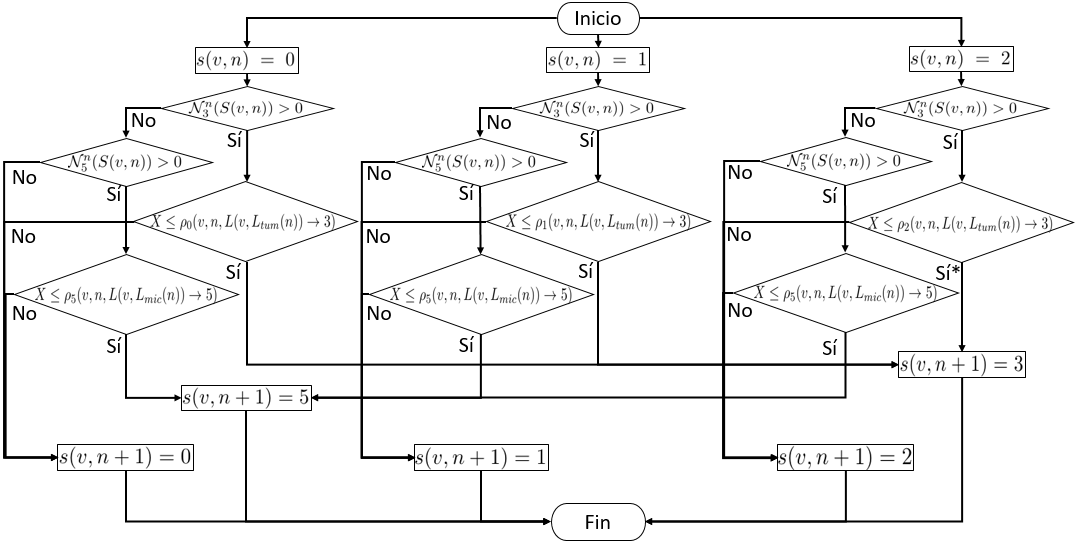
\includegraphics{img/fig-flux-diagram.png}}
\end{center}
\caption[Diagrama de flujo de las reglas del crecimiento tumoral y del crecimiento de las micromet\'astasis]{Diagrama de flujo de las reglas del crecimiento tumoral y del crecimiento de las micromet\'astasis. Se aprecian las distintas rutas que pueden tomar las c\'elulas normales del modelo para cambiar su estado al de una c\'elula cancer\'igena tumoral o a la de una micromet\'astasis en dependencia de las condiciones de su vecindad y del c\'alculo de las probabilidades de transici\'on. \textit{En el diagrama:} (*) Solo existen probabilidades de que ocurra durante la etapa vascular.}
\label{fig-flux-diagram}
\end{figure}

\subsubsection*{Reglas de la cascada metast\'asica}
 En las secciones~\ref{subsec-migrant}, \ref{subsec-migration} y \ref{subsec-metastasis} se sigui\'o un proceso gradual para la obtenci\'on de las reglas que representan la cascada metast\'asica, desde la aparici\'on de las c\'elulas migratorias, su desplazamiento a trav\'es del estroma, el transporte a trav\'es del sistema circulatorio y la creaci\'on de una nueva micromet\'astasis. A continuaci\'on se presenta un resumen de las reglas mencionadas de forma tal que se muestren como componentes integradores de la funci\'on de transici\'on local. Se expondr\'an las definiciones e hip\'otesis que se tuvieron en cuenta en cada caso para una r\'apida referencia. De esta forma tenemos el conjunto de reglas que reproducen la cascada metast\'asica como: 
\begin{equation*}
s(v,n+1)=\mathcal{R}(S(v,n))=\left\lbrace
	\begin{array}{ll}
		\zeta_2(v,n,L(v,L_{tum}(n))) & \textit{si } s(v,n)=2~\wedge~\mathcal{N}_3^n(S(v,n)) > 0 \\[0.2cm]
		\zeta_4(\mu(v,n)) & \textit{si } s(v,n)=4~\wedge~\mathcal{N}_{\mathcal{E}_{met}}^d(S(v,n))=0~\wedge\\
				         & \mathcal{N}_2^n(S(v,n))=0 \\
		2 & \textit{si } s(v,n)=4~\wedge~\mathcal{N}_{\mathcal{E}_{met}}^d(S(v,n))=0~\wedge\\
		  & \mathcal{N}_2^n(S(v,n))>0 \\[0.2cm]
		2 & \textit{si } s(v,n)=4~\wedge~\mathcal{N}_{\mathcal{E}_{met}}^d(S(v,n))>0
	\end{array}
\right..
\end{equation*}

La primera de estas reglas se corresponde con el \emph{surgimiento de c\'elulas migratorias}, de la que se realizan las siguientes anotaciones:\label{NOT-surgimiento-celulas-migratorias}

\paragraph*{{Fundamento biol\'ogico}:} La acumulaci\'on de mutaciones de las c\'elulas cancer\'igenas y los cambios en la matriz de interacci\'on intercelular provocados por la angiog\'enesis tumoral hacen posible que aparezcan c\'elulas con una reducida adhesi\'on celular y que expresan prote\'inas involucradas en el control de la movilidad y la supresi\'on de reguladores de la migraci\'on. Estos cambios solo se expresan en la etapa vascular del desarrollo tumoral. En la concepci\'on de estas reglas se adoptan de forma general las hip\'otesis I, II y VI que tratan sobre la progresi\'on idealizada del desarrollo tumoral, las mutaciones de las c\'elulas cancer\'igenas y la homogeneidad de las c\'elulas cancer\'igenas respectivamente.

\paragraph*{{Criterio de selecci\'on}:} Una c\'elula normal que pertenece al estroma expresado mediante la condici\'on $s(v,n)=2$ tiene una posibilidad de cambiar su estado al de una c\'elula migratoria del c\'ancer si en su vecindad inmediata existen c\'elulas pertenecientes a alg\'un tumor, expresado mediante la condici\'on $\mathcal{N}_3^n(S(v,n))>0$. Las funciones utilizadas son definidas en~\ref{def-cellstatus} y \ref{def-near-neighbours} respectivamente.

\paragraph*{{Funcionamiento}:} Para representar el surgimiento de estas c\'elulas hacemos que la variable aleatoria utilizada para reproducir la expansi\'on tumoral hacia el estroma pueda tomar el estado correspondiente con el de una c\'elula migratoria. De esta forma cuando el tumor est\'a en las \'ultimas instancias de su desarrollo en la etapa vascular al este crecer existe la posibilidad de que las nuevas c\'elulas cancer\'igenas se correspondan con el tipo migratorio. Luego si el criterio de selecci\'on de la regla se cumple, el valor del estado de la c\'elula $v$ en el instante de tiempo $n+1$ se determina a trav\'es de la variable aleatoria $\zeta_2(v,n,L(v,L_{tum}(n)))$ que puede tomar los valores:
\begin{align*}
\zeta_2(v,n,L(v,L_{tum}(n))) &\in \lbrace 2,3,4 \rbrace.
\end{align*}
Esta variable aleatoria posee la siguiente distribuci\'on de probabilidad:
\begin{align*}
P(\zeta_2(v,n,L(v,L_{tum}(n)))=2) &= 1 - \left[\rho_2(v,n,L(v,L_{tum}(n)) \rightarrow 3) + \rho_2(L(v,L_{tum}(n)) \rightarrow 4)\right], \\
P(\zeta_2(v,n,L(v,L_{tum}(n)))=3) &= \rho_2(v,n,L(v,L_{tum}(n)) \rightarrow 3), \\
P(\zeta_2(v,n,L(v,L_{tum}(n)))=4) &= \rho_2(L(v,L_{tum}(n)) \rightarrow 4).
\end{align*}
La probabilidad de transici\'on $\rho_2(v,n,L(v,L_{tum}(n)) \rightarrow 3)$ se utiliza para reproducir la expansi\'on tumoral, como se mostr\'o anteriormente, mientras que $\rho_2(L(v,L_{tum}(n)) \rightarrow 4)$ se utiliza para reproducir el surgimiento de c\'elulas migratorias. La extensi\'on de la concepci\'on cl\'asica de un aut\'omata celular que permite el uso de estas probabilidades de transici\'on se presenta en las definici\'on~\ref{prop-newlocal-func-3}. La expresi\'on para el c\'alculo de esta probabilidad de transici\'on, de acuerdo a la hip\'otesis XV sobre las situaciones de competencia entre tumores, se muestra a continuaci\'on:
\begin{equation*}
\rho_2(L(v,L_{tum}(n)) \rightarrow 4) = max\left[\rho_2(l_1 \rightarrow 4),\,\rho_2(l_2 \rightarrow 4),\ldots,\,\rho_2(l_m \rightarrow 4)\right].
\end{equation*}
En la expresi\'on anterior la funci\'on $L(v,L_{tum}(n))$ devuelve los tumores vecinos a la c\'elula $v$, como se muestra en la definici\'on~\ref{def-L-2}, donde $L_{tum}(n)$ contiene a las c\'elulas que forman cada tumor en la simulaci\'on, como se muestra en la definici\'on~\ref{def-L-n}. De ah\'i que $L(v,L_{tum}(n))=\lbrace l_1, l_2, \ldots, l_m \rbrace$ con $m=|L(v,L_{tum}(n))|$. De acuerdo a las hip\'otesis VIII y XIV sobre el desarrollo tumoral en funci\'on de la poblaci\'on y la interpretaci\'on de la neovasculatura respectivamente el c\'alculo de las probabilidades particulares $\rho_2(l \rightarrow 4)$ para cada tumor $l \in L(v,L_{tum}(n))$ se realiza mediante la expresi\'on siguiente:
\begin{equation*}
\rho_2(l \rightarrow 4) = (1-H(l,P_0^v)) \left( \displaystyle\frac{|l|}{K_v + K_{mig}} \right)^{\displaystyle 1/\eta_{mig}}.
\end{equation*}
Los par\'ametros $\eta_{mig} \in (0,1]$ y $K_{mig} \in \mathbb{N}$ nos permiten ajustar el comportamiento de la regla. Mediante la variaci\'on de $\eta_{mig}$ se puede variar el instante de tiempo en el que comienza el surgimiento de c\'elulas migratorias y la variaci\'on de $K_{mig}$ permite establecer un l\'imite para la probabilidad de surgimiento de dichas c\'elulas migratorias.\vspace*{0.5cm}

La segunda y tercera de estas reglas se corresponden con la \emph{migraci\'on}, de la que se realizan las siguientes anotaciones:\label{NOT-migracion}

\paragraph*{{Fundamento biol\'ogico}:} Una c\'elula cancer\'igena migratoria habiendo ingresado en el estroma procede a desplazarse a trav\'es del tejido mediante la degradaci\'on progresiva de la ECM hasta penetrar el sistema circulatorio en un posible punto de inserci\'on. El desplazamiento se produce aumentando progresivamente la distancia existente entre la c\'elula migratoria y la masa tumoral de la que se desprendi\'o porque esta toma la mayor\'ia de los nutrientes del entorno circundante y lo hace avanzando hacia la direcci\'on de donde provienen los nutrientes de la difusi\'on. Durante la migraci\'on existen tres situaciones fundamentales que pueden ocurrir: que la c\'elula migratoria posea destinos viables hacia los que desplazarse, que la c\'elula migratoria est\'e inm\'ovil y que la c\'elula migratoria est\'e en posici\'on de penetrar el sistema circulatorio ya que se encuentra en un posible punto de inserci\'on. La \'ultima situaci\'on se corresponde con el fin de la migraci\'on expresada en la cuarta regla relacionada con la cascada metast\'asica como se expondr\'a posteriormente. La concepci\'on de estas reglas se apoya en las hip\'otesis XVIII y XIX sobre la migraci\'on del c\'ancer y el sesgo direccional de la migraci\'on respectivamente.

\paragraph*{{Criterio de selecci\'on}:} Una c\'elula migratoria, expresado por la condici\'on $s(v,n)=4$, que no est\'e en posici\'on de penetrar el sistema circulatorio, expresado por la condici\'on $\mathcal{N}_{\mathcal{E}_{met}}^d(S(v,n))=0$ donde $\mathcal{E}_{met}=\lbrace 2,3,5 \rbrace$ son los destinos posibles de una met\'astasis, puede encontrarse en dos situaciones fundamentales: que est\'e inm\'ovil, expresado por la condici\'on $\mathcal{N}_2^n(S(v,n))=0$ en la segunda regla de la migraci\'on, o que posea destinos viables hacia los que desplazarse, expresado por la condici\'on $\mathcal{N}_2^n(S(v,n))>0$ en la tercera regla de la migraci\'on. Las funciones utilizadas son definidas en~\ref{def-cellstatus}, \ref{def-near-neighbours} y \ref{def-normal-distant-neighbours} respectivamente.

\paragraph*{{Funcionamiento}:} La actualizaci\'on de las c\'elulas migratorias en el presente aut\'omata celular se lleva a cabo en el m\'etodo $update-migratory-cells(G,\,C_{mig}^A(G),\,S(n),$ $\psi_{mig},\,\mu_{mig})$, mostrado en esta secci\'on en el algoritmo~\ref{alg-update-r-2}, en el que el orden en que son seleccionadas estas c\'elulas es aleatorio dada la naturaleza as\'incrona de la actualizaci\'on, donde los par\'ametros $\psi_{mig} \in [0,1]$ y $\mu_{mig} \in \mathbb{N}$ que se corresponden con una probabilidad de llevar a cabo un movimiento y el rango m\'aximo del propio movimiento respectivamente permiten la reproducci\'on de forma m\'as realista del movimiento de las c\'elulas cancer\'igenas, permitiendo desplazamientos con rangos variables, adem\'as de proporcionar un nuevo grado de ajuste al modelo. En caso de que se aplique la \emph{segunda regla} correspondiente con la de una c\'elula migratoria inm\'ovil se prueba su supervivencia haciendo el estado de la posici\'on actual igual al de la variable aleatoria $\zeta_4(\mu(v,n))$:
\begin{equation*}
s(v,n+1) = \zeta_4(\mu(v,n)).
\end{equation*}
Esta variable aleatoria puede tomar los siguientes valores:
\begin{equation*}
\zeta_4(\mu(v,n)) \in \lbrace 2,4 \rbrace.
\end{equation*}
Si toma valor $2$ se asume que la existencia de la c\'elula migratoria termin\'o y la posici\'on dejada por ella es ocupada por el estroma. Si toma valor $4$ la c\'elula migratoria contin\'ua con su existencia pero permanece inm\'ovil. Posee la siguiente distribuci\'on de probabilidad:
\begin{align*}
P(\zeta_4(\mu(v,n))=2) &= \rho_4(\mu(v,n) \rightarrow 2), \\
P(\zeta_4(\mu(v,n))=4) &= 1 - \rho_4(\mu(v,n) \rightarrow 2).
\end{align*}
La probabilidad de transici\'on $\rho_4(\mu(v,n) \rightarrow 2)$ se utiliza para determinar la supervivencia de la c\'elula migratoria. La extensi\'on de la concepci\'on cl\'asica de un aut\'omata celular que permite el uso de estas probabilidades de transici\'on se presenta en las definici\'on~\ref{prop-newlocal-func-4}. Se expresa como el cociente entre la distancia recorrida, determinada mediante la funci\'on $\mu(v,n)$, y la distancia promedio m\'axima $\mu_{max} \in \mathbb{N}$, es decir:
\begin{equation*}
\rho_4(\mu(v,n) \rightarrow 2) = \left(\displaystyle\frac{\mu(v,n)}{\mu_{max}} \right)^{\displaystyle 1 / \eta_{mig}'}.
\end{equation*}
El par\'ametro $\eta_{mig}' \in (0,1]$ nos permite ajustar el comportamiento de la regla. Mediante la variaci\'on de $\eta_{mig}'$ se pueden representar condiciones favorables o adversas para la supervivencia de la c\'elula migratoria. En caso de que se aplique la \emph{tercera regla} correspondiente con la existencia de destinos viables en la migraci\'on se utiliza una t\'ecnica conocida como intercambio de estados en teor\'ia de aut\'omatas celulares donde al actualizarse una part\'icula en movimiento se actualizan los estados de la posici\'on inicial y la final simult\'aneamente. El procedimiento se resume como: $(1)$ se le asigna a la posici\'on inicial $v$ de la c\'elula migratoria el estado $2$ mediante la aplicaci\'on de la regla; $(2)$ se selecciona una posici\'on destino $w$ mediante la aplicaci\'on de la funci\'on $d_{mig}(v,n)$; y $(3)$ se le asigna a la posici\'on destino elegida $w$ de la c\'elula migratoria el estado que tome la variable aleatoria $\zeta_4(\mu(v,n))$. Si la posici\'on destino toma el estado $2$ se considera que termin\'o la existencia de la c\'elula migratoria, en caso contrario si toma el estado $4$ se considera que el desplazamiento fue satisfactorio y la c\'elula contin\'ua con su existencia. La funci\'on $d_{mig}(v,n)$, definida en~\ref{def-dest-selection-2}, se plantea como:
\begin{equation*}
d_{mig}(v,n) = \left\lbrace
	\begin{array}{ll}
		v & \textit{si } |D_{mig}(v,n)|=0\\
		d_{mig}'(v,n) & \textit{si } |D_{mig}(v,n)|\neq 0		
	\end{array}
\right.. 
\end{equation*}
La funci\'on $D_{mig}(v,n)$, definida en~\ref{def-type-neighbours} devuelve los posibles destinos a los que puede desplazarse la c\'elula migratoria en cuesti\'on, siempre y cuando estos destinos la alejen del tumor donde se origin\'o, es decir:
\begin{equation*}
D_{mig}(v,n) = \lbrace w~|~w \in \mathcal{N}^n(v)~\wedge~s(w,n)=2~\wedge~o(v) = o(w)~\wedge~d_E(c_l,w) > d_E(c_l,v) \rbrace.
\end{equation*}
Si $d_{mig}(v,n) = v$ es porque no existen destinos viables hacia los que realizar la migraci\'on expresado por la condici\'on $|D_{mig}(v,n)|=0$, en caso contrario si $D_{mig}(v,n)= \lbrace w_1,w_2,\ldots,w_m \rbrace$ con $m = |D_{mig}(v,n)|$, es decir $|D_{mig}(v,n)|\neq 0$, el destino se elige mediante la funci\'on $d_{mig}'(v,n)$, que posee la siguiente expresi\'on:
\begin{equation*}
d_{mig}'(v,n) = \left\lbrace
	\begin{array}{ll}
		w_1 & \textit{con probabilidad } \frac{1}{m} \beta_{mig}(v,w_1)\\
		w_2 & \textit{con probabilidad } \frac{1}{m} \beta_{mig}(v,w_2)\\
		\vdots & \ldots\\
		w_m & \textit{con probabilidad } \frac{1}{m} \beta_{mig}(v,w_m)
	\end{array}\
\right..
\end{equation*}
Como se puede apreciar la probabilidad de que una posici\'on destino sea elegida satisfactoriamente depende de la funci\'on $\beta_{mig}(v,w)$, definida en~\ref{def-dest-selection}, y constituye de acuerdo a la hip\'otesis XIX sobre el sesgo direccional de la migraci\'on una forma de hacer que la migraci\'on se desarrolle hacia la vasculatura. Finalmente la posici\'on inicial $v$ y la posici\'on destino $w$ se actualizan con los valores correspondientes de acuerdo a lo planteado anteriormente:
\begin{align*}
s(v,n+1) &= 2,\\
s(w,n+1) &= \zeta_4(\mu(v,n)). 
\end{align*}\vspace*{0.5cm}

La regla final se corresponde con la \emph{met\'astasis}, de la que se realizan las siguientes anotaciones:\label{NOT-metastasis}

\paragraph*{{Fundamento biol\'ogico}:} Una c\'elula cancer\'igena migratoria que est\'e en presencia de un posible punto de intravasaci\'on procede a penetrar el sistema circulatorio para dar continuaci\'on a la cascada metast\'asica. Durante la estancia en el sistema circulatorio su existencia puede ser terminada por el sistema inmunitario o como consecuencia del estr\'es mec\'anico sufrido. Eventualmente se adhieren a un posible punto de extravasaci\'on en el que degradan la pared del vaso sangu\'ineo y abandona el sistema circulatorio. La concepci\'on de esta regla se apoya en las hip\'otesis XX y XXI sobre las conexiones distantes del grafo y los destinos viables de la met\'astasis.

\paragraph*{{Criterio de selecci\'on}:} Una c\'elula migratoria, expresado por la condici\'on $s(v,n)=4$, que est\'e en posici\'on de penetrar el sistema circulatorio, expresado por la condici\'on $\mathcal{N}_{\mathcal{E}_{met}}^d(S(v,n))>0$ donde $\mathcal{E}_{met}=\lbrace 2,3,5 \rbrace$ son los destinos posibles de una met\'astasis, abandona su posici\'on y pasa a pertenecer al conjunto de actualizaci\'on as\'incrono $C_{sc}^A(G)$ donde permanecer\'a por un per\'iodo de tiempo, hasta que lo abandone satisfactoriamente en la posici\'on destino.

\paragraph*{{Funcionamiento}:} La penetraci\'on del sistema circulatorio puede ocurrir en dos localizaciones: en un capilar sangu\'ineo distante de la masa tumoral al que arriban las c\'elulas cancer\'igenas despu\'es de llevar a cabo la migraci\'on a trav\'es del estroma, y en un capilar sangu\'ineo que pertenezca al interior del tumor producto de la angiog\'enesis. La primera de estas situaciones es tratada mediante la regla de la met\'astasis que se expone a continuaci\'on, mientras que la segunda situaci\'on se trata mediante el m\'etodo $update-tumor-migratory-cells(G,\,C_{tum}^A(G),\,C_{sc}^A(G),\,S(n))$ del procedimiento de actualizaci\'on, presentado en esta secci\'on en~\ref{alg-update-r-3}. La regla es determinista en el sentido de que si se cumple el criterio de selecci\'on, la c\'elula migratoria siempre abandona su posici\'on y penetra el sistema circulatorio, es decir, pasa a pertenecer al conjunto de actualizaci\'on as\'incrono $C_{sc}^A(G)$ con la informaci\'on referente a su destino y con un tiempo de transporte igual a cero. El destino de la met\'astasis se elige de forma aleatoria a trav\'es de la funci\'on $d_{met}(v,n)$, definida en~\ref{def-dest-selection-met}, cuya expresi\'on es la siguiente:
\begin{figure}[t!]
\begin{center}
\scalebox{0.52}{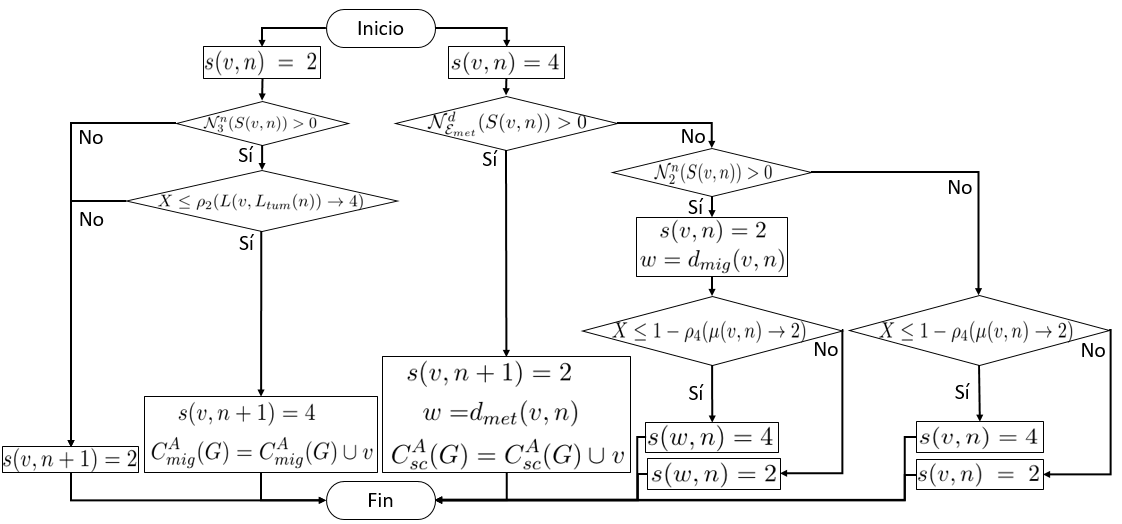
\includegraphics{img/fig-flux-diagram-2.png}}
\end{center}
\caption[Diagrama de flujo de las reglas de la aparici\'on de c\'elulas migratorias, migraci\'on y met\'astasis]{Diagrama de flujo de las reglas de la aparici\'on de c\'elulas migratorias, migraci\'on y met\'astasis. Se aprecian la situaci\'on que provoca la aparici\'on de c\'elulas migratorias en la frontera del tumor, las situaciones que pueden darse durante la migraci\'on de estas c\'elulas cancer\'igenas y algunos detalles de c\'omo se lleva a cabo la selecci\'on de los destinos de la misma y de la met\'astasis.}
\label{fig-flux-diagram-2}
\end{figure}
\begin{equation*}
d_{met}(v,n) = \left\lbrace
	\begin{array}{ll}
		w_1 & \textit{con probabilidad } 1/m\\
		w_2 & \textit{con probabilidad } 1/m\\
		\vdots & \ldots\\
		w_m & \textit{con probabilidad } 1/m
	\end{array}
\right..
\end{equation*}
La funci\'on $D_{met}(v,n)$, definida en~\ref{def-type-neighbours-2}, que devuelve el conjunto compuesto por los posibles destinos de la met\'astasis $\lbrace w_1, w_2, \ldots, w_m \rbrace$ con $m = |D_{met}(v,n)|$ posee la siguiente expresi\'on:
\begin{equation*}
D_{met}(v,n) = \lbrace w~|~w \in \mathcal{N}^d(v)~\wedge~s(w,n) \in \mathcal{E}_{met} \rbrace.
\end{equation*}
El m\'etodo $update-tumor-migratory-cells(G,\,C_{tum}^A(G),\,C_{sc}^A(G),\,S(n))$ es an\'alogo al proceso realizado por la migraci\'on: el orden de actualizaci\'on se define de forma aleatoria, se eval\'ua la probabilidad de que la c\'elula tumoral que est\'a en presencia del capilar sangu\'ineo produzca una descendencia migratoria mediante el m\'etodo $get-probability(v)$ equivalente a la funci\'on $\rho_2(l \rightarrow 4)$ definida en~\ref{eq-migrant-2} y \ref{eq-migrant-3}, se selecciona el destino de la met\'astasis mediante el m\'etodo $select-destiny-vertex(v,\,S(n),\,G)$ equivalente a la funci\'on $d_{met}(v,n)$, y finalmente se a\~nade la descendencia migratoria al sistema circulatorio mediante el m\'etodo $add-cell-to-bloodstream(v,\,d,\,C_{sc}^A(G))$. El m\'etodo $update-migratory-cells-in-bloodstream(C_{sc}^A(G),\,\psi_{met0},\,\psi_{met1},\,T_{sc},\,\xi_{sc})$, presentado en esta secci\'on en~\ref{alg-update-r-1}, es el encargado de actualizar el conjunto as\'incrono $C_{sc}^A(G)$ que contiene las c\'elulas migratorias que residen en el torrente sangu\'ineo, evaluando su supervivencia y su arribo a la localizaci\'on destino, determinando si se crea satisfactoriamente una nueva micromet\'astasis. En la figura~\ref{fig-flux-diagram-2} se representan las reglas de la migraci\'on y met\'astasis en un diagrama de flujo. Al igual que en el diagrama de flujo de las reglas de la conservaci\'on del estado de las c\'elulas normales, del crecimiento tumoral y del crecimiento de las micromet\'astasis, se utiliza una variable aleatoria $X$ que posee una distribuci\'on uniforme en $[0,1]$. 